To edit what the games does and how they look like we wanted meant that a lot of variables from our scripts had to be exposed.
By default Unity will expose all public variables in a script.
This includes scripts that the script want publicly available for other scripts to get or variables that should not be accessible for the
user but accessible for other scripts as the variable is only kept in the script but not used.

In our case we had a script that was to hold as much data about a minigame as possible.
This was so the game could be easily changed in the inspector of Unity without having to go into a script and manually edit.

The inspector quickly became crowded both by unnecessary variables that while they were needed they were not needed exposed all the time.
For instance there is no need to see the variables for creating a grid when you are creating a shape matching game.
And with the possibility of creating any of the minigames that we have implemented when you are creating a new game in a new scene in Unity 
this will lead to quite a lot of variables being exposed even if we try to share as many variables as possible.

To solve this problem we created a script to interact with the editor side of Unity to tell Unity how we
want the editor to look like instead of using the default behavior.
Doing it this way meant that we would have complete control over what is displayed and how.
Having complete control also means that we had to explicitly tell Unity what variables should go where, what name to show
for the field in the inspector, what values was acceptable and so on. 

\begin{wrapfigure}{l}{0.47\textwidth}
	\capstart
	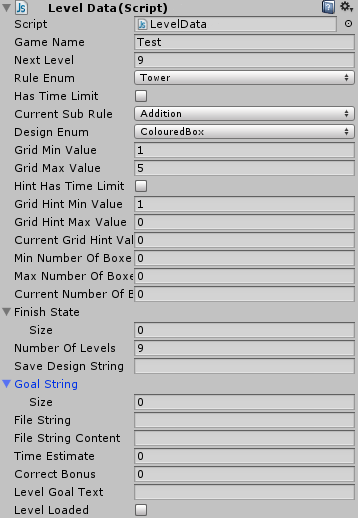
\includegraphics[width=0.45\textwidth]{images/inspector.png}
	\caption{Default Unity inspector}
\end{wrapfigure}

\begin{wrapfigure}{r}{0.47\textwidth}
	\capstart
	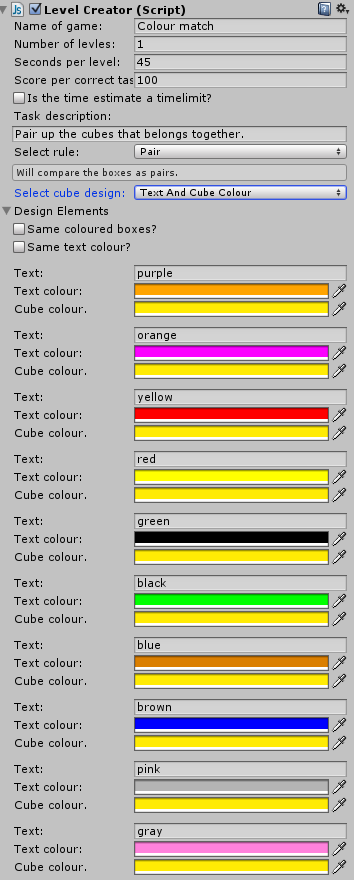
\includegraphics[width=0.45\textwidth]{images/inspector edited.png}
	\caption{cogArc custom inspector}
\end{wrapfigure}

Seen above are the data with the default inspector in Unity, what is not seen is the data about how cubes should look as this data 
is not in a format that Unity can show.
The other picture shows the inspector we built. 
Our inspector hides variables that is either not needed with the current settings or is not for the user to temper with.
This makes it easy to manipulate already made scenes / minigames in Unity or to swiftly create a new variant of a minigame.
And testing new configurations is quick and easy as all values and inputs are constricted to be only acceptable values.
This alleviates the user from a lot of respocibility and having to know about what goes on when data is changed as all of this is automated.
